%%%%%%%%%%%%%%%%%%%%%%%%%%%%%%%%%%%%%%%%%%%%%%%%
%
% This is file life_mix_phis.tex containing
% the subsection about the phi_s
%
%%%%%%%%%%%%%%%%%%%%%%%%%%%%%%%%%%%%%%%%%%%%%%%
%

%---------------------------------------------
% \subsubsubsection{Weak phase in \Bs mixing}
%---------------------------------------------
\labs{phasebs}

%%% \noindent
%%% \fbox{\parbox{\textwidth}{{\bf WARNING}: Several new results became available but are not yet included in the averages, plots, tables and discussion of this paragraph. These include:
%%% \newline$\bullet$ a finalized version of the analysis described in note ATLAS-CONF-2013-039~\cite{Aad:2014cqa,*Aad:2012kba_cont}; 
%%% \newline$\bullet$ a preliminary $\B_s \to\jpsi\phi$ analysis from CMS~\cite{CMS-PAS-BPH-13-012};
%%% \newline$\bullet$ a new $\phi_s$ result with $B^0_s\to\jpsi\pi^+\pi^-$ from LHCb~\cite{Aaij:2014dka,*Aaij:2013oba_supersede};
%%% \newline$\bullet$ a new $\phi_s$ result with $B^0_s\to\jpsi K^+K^-$ from LHCb~\cite{Aaij:2014zsa,*Aaij:2013oba_supersede2};
%%% \newline$\bullet$ a new $\phi_s$ result with $\bar{B}^0_s\to D_s^+D_s^-$ decays from LHCb~\cite{Aaij:2014ywt}.
%%% \newline These new results have been added to \Table{phisDGsGs}, but otherwise the text has not been updated.
%%% }}
%%% \marginpar{XXX}

\CP violation induced by $\Bs-\Bsbar$ mixing
% in $b \to c\bar{c}s$ decays
has been a field of 
very active study and fast experimental progress 
in the past couple of years.
%OS% Similarly to what has happened at the \B factories 
%OS% a decade ago, when the \Bd mixing-induced phase $2\beta$
%OS% was measured, the Tevatron and LHC experiments are 
%OS% now obtaining point estimates
%OS% of the \Bs mixing-induced phase \phiccbars.
The main observable is the 
\CP-violating phase \phiccbars, defined as 
the weak phase difference between
the $\Bs-\Bsbar$ mixing amplitude
and the $b \to c\bar{c}s$ decay amplitude.

The golden mode for such studies is 
$\Bs \to \jpsi\phi$, followed by $\jpsi \to \mu^+\mu^-$ and 
$\phi\to K^+K^-$, for which a full angular 
analysis of the decay products is performed to 
separate statistically the \CP-even and \CP-odd
contributions in the final state. As already mentioned in 
\Sec{DGs},
CDF~\cite{Aaltonen:2012ie,*CDF:2011af,*Aaltonen:2007he_mod,*Aaltonen:2007gf_mod},
\dzero~\cite{Abazov:2011ry,*Abazov_mod:2008fj,*Abazov:2007tx_mod_cont},
ATLAS~\cite{Aad:2014cqa,*Aad:2012kba_cont}, CMS~\cite{CMS-PAS-BPH-13-012}
and LHCb~\cite{Aaij:2014zsa,*Aaij:2013oba_supersede2}
have used both untagged and tagged $\Bs \to \jpsi\phi$ (and $\Bs \to \jpsi K^+K^-$) events 
for the measurement of \phiccbars.
LHCb~\cite{Aaij:2014dka,*Aaij:2013oba_supersede}
has used $\Bs \to \jpsi \pi^+\pi^-$ events, 
analyzed with a full amplitude model
including several $\pi^+\pi^-$ resonances (\eg $f_0(980)$),
although the
$\jpsi \pi^+\pi^-$ final state had already been shown
to be almost \CP pure with a \CP-odd fraction
larger than 0.977 at 95\% CL~\cite{LHCb:2012ae}. 
In addition, LHCb has used the $\Bs \to \Dsp\Dsm$ channel~\cite{Aaij:2014ywt} to measure \phiccbars.

All CDF, \dzero, ATLAS and CMS analyses provide 
two mirror solutions related by the transformation 
$(\DGs, \phiccbars) \to (-\DGs, \pi-\phiccbars)$. However, the
LHCb analysis of $\Bs \to \jpsi K^+K^-$ resolves this ambiguity and 
rules out the solution with negative \DGs~\cite{Aaij:2012eq},
a result in agreement with the Standard Model expectation.
Therefore, in what follows, we only consider the solution with $\DGs > 0$.

%% Text from OL:
%%% The relative phase between the \Bs mixing amplitude and that of
%%% specific $b \to c\bar{c}s$ quark transitions such as 
%%% for \Bs or \Bsbar $\to \jpsi \phi$,
%%% is called \phiccbars. %~\cite{Lenz:2011ti,*Lenz:2006hd,Charles:2011va_mod,*Bona:2006ah}: 

%OLD% \begin{table}
%OLD% \caption{Direct experimental measurements of \phiccbars, \DGs and \Gs using
%OLD% $\Bs\to\jpsi\phi$, $\Bs\to\jpsi K^+K^-$ and $\Bs\to\jpsi\pi^+\pi^-$ decays.
%OLD% Only the solution with $\DGs > 0$ is shown, since the two-fold ambiguity has been
%OLD% resolved in \Ref{Aaij:2012eq}. The first error is due to 
%OLD% statistics, the second one to systematics. The last line gives our average.}
%OLD% \labt{phisDGsGs}
%OLD% \begin{center}
%OLD% \begin{tabular}{@{}l@{\,}l@{\,}l@{\,}|@{\,}l@{\,}|@{\,}l@{\,}|@{\,}l@{}} 
%OLD% \hline
%OLD% Exp.\ & Mode & Ref.\ & \multicolumn{1}{c@{\,}|@{\,}}{\phiccbars}
%OLD%                      & \multicolumn{1}{c@{\,}|@{\,}}{\DGs (\!\!\invps)}
%OLD%                      & \multicolumn{1}{c@{}}{\Gs (\!\!\invps)} \\ 
%OLD% \hline
%OLD% CDF    & $\jpsi\phi$ & \cite{Aaltonen:2012ie,*CDF:2011af,*Aaltonen:2007he_mod,*Aaltonen:2007gf_mod}
%OLD%        & $[-0.60,\, 0.12]$, 68\% CL & $0.068\pm0.026\pm0.009$ % syst error was +-0.007 instead of +-0.009 in CDF note 10778
%OLD%        & $0.654\pm0.008\pm0.004$ \\ % quoted in paper as tau(Bs) = 1/Gamma_s = 1.528 +-0.019 +-0.009
%OLD% % 1./1.528 = 0.6544502617801047, 0.019/1.528**2 = 0.008137797757736905, 0.009//1.528**2 = 0.003854746306296428
%OLD% \dzero & $\jpsi\phi$ & \cite{Abazov:2011ry,*Abazov_mod:2008fj,*Abazov:2007tx_mod_cont}
%OLD%        & $-0.55^{+0.38}_{-0.36}$ & $0.163^{+0.065}_{-0.064}$ & $0.693^{+0.018}_{-0.017}$  \\
%OLD% ATLAS  & $\jpsi\phi$ & \cite{Aad:2014cqa,*Aad:2012kba_cont}
%OLD%        & $+0.12 \pm 0.25 \pm 0.05$ & $0.053 \pm0.021 \pm0.010$ & $0.677 \pm0.007 \pm0.004$ \\
%OLD% %%% CMS    & $\jpsi\phi$ & \cite{CMS-PAS-BPH-11-006}$^p$   % this CMS result not included in the (phi_s, DGs) averaging !
%OLD% %%%        & (set to $0$) & $0.048\pm0.024\pm0.003$ & --- \\
%OLD% CMS    & $\jpsi\phi$ & \cite{CMS-PAS-BPH-13-012}$^p$
%OLD%        & $-0.03 \pm 0.11 \pm 0.03$ & $0.096\pm0.014\pm0.007$ & $0.670 \pm0.004 \pm0.005$ \\
%OLD% %%% the CMS note CMS-PAS-BPH-13-012 quote a "mean Bs lifetime" of
%OLD% %%%    ctau = 447.3 +-3.0 +-3.5 microns = 1.492 +-0.010 +-0.012 ps
%OLD% %%%    corresponding to Gamma_s = 0.6702 +-0.0045 +-0.0052 ps-1
%OLD% LHCb   & $\jpsi KK$ & \cite{Aaij:2014zsa,*Aaij:2013oba_supersede2}
%OLD%        & $-0.058\pm0.049\pm0.006$ & $0.0805\pm0.0091\pm0.0033$ & $0.6603\pm0.0027\pm0.0015$  \\
%OLD% LHCb   & $\jpsi\pi\pi$ & \cite{Aaij:2014dka,*Aaij:2013oba_supersede}
%OLD%        & $+0.070 \pm0.068 \pm 0.008$ & --- & --- \\
%OLD% LHCb   & $\jpsi hh$ & \cite{Aaij:2014zsa,*Aaij:2013oba_supersede2}
%OLD%        & $-0.010\pm0.040(\rm tot)$ & --- & --- \\
%OLD% LHCb   & $D_sD_s$ & \cite{Aaij:2014ywt}
%OLD%        & $+0.02 \pm0.17 \pm 0.02$ & --- & --- \\
%OLD% %old%LHCb   & $\jpsi KK$ & \cite{Aaij:2013oba,*LHCb:2011aa_mod,*LHCb:2012ad_mod,*LHCb:2011ab_mod,*Aaij:2012nta_mod}
%OLD% %old%       & $+0.07\pm0.09\pm0.01$ & $0.100\pm0.016\pm0.003$ & $0.663\pm0.005\pm0.006$  \\
%OLD% %old%LHCb   & $\jpsi\pi\pi$ & \cite{Aaij:2013oba,*LHCb:2011aa_mod,*LHCb:2012ad_mod,*LHCb:2011ab_mod,*Aaij:2012nta_mod}
%OLD% %old%       & $-0.014 ^{+0.17}_{-0.16}\pm 0.01$ & --- & --- \\
%OLD% %old%LHCb   & combined & \cite{Aaij:2013oba,*LHCb:2011aa_mod,*LHCb:2012ad_mod,*LHCb:2011ab_mod,*Aaij:2012nta_mod}
%OLD% %old%       & $+0.01\pm0.07\pm0.01$ & $0.106\pm0.011\pm0.007$ & $0.661\pm0.004\pm0.006$  \\
%OLD% \hline
%OLD% \multicolumn{3}{@{}l@{\,}|@{\,}}{All combined} & \hfagPHISCOMB & \hfagDGSCOMBnounit & \hfagGSnounit \\
%OLD% \hline
%OLD% \multicolumn{6}{l}{$^p$ {\footnotesize Preliminary.}}
%OLD% \end{tabular}
%OLD% \end{center}
%OLD% \end{table}

\begin{table}
\caption{Direct experimental measurements of \phiccbars, \DGs and \Gs using
$\Bs\to\jpsi\phi$, $\jpsi K^+K^-$, $\jpsi\pi^+\pi^-$ and $D_s^+D_s^-$ decays.
Only the solution with $\DGs > 0$ is shown, since the two-fold ambiguity has been
resolved in \Ref{Aaij:2012eq}. The first error is due to 
statistics, the second one to systematics. The last line gives our average.}
\labt{phisDGsGs}
\begin{center}
%\begin{tabular}{l@{\,}l@{\,}l@{\,}|@{\,}l@{\,}|@{\,}l@{\,}|@{\,}l} 
\begin{tabular}{llrlll} 
\hline
% Exp.\ & Mode & Dataset & \multicolumn{1}{c@{\,}|@{\,}}{\phiccbars}
%                      & \multicolumn{1}{c@{}}{\DGs (\!\!\invps)} & Ref.\ \\
Exp.\ & Mode & Dataset & \multicolumn{1}{c}{\phiccbars}
                     & \multicolumn{1}{c}{\DGs (\!\!\invps)} & Ref.\ \\
\hline
CDF    & $\jpsi\phi$ & $9.6\invfb$
       & $[-0.60,\, 0.12]$, 68\% CL & $0.068\pm0.026\pm0.009$
       & \cite{Aaltonen:2012ie,*CDF:2011af,*Aaltonen:2007he_mod,*Aaltonen:2007gf_mod} \\
       % syst error was +-0.007 instead of +-0.009 in CDF note 10778
       % & $0.654\pm0.008\pm0.004$ \\ % quoted in paper as tau(Bs) = 1/Gamma_s = 1.528 +-0.019 +-0.009
% 1./1.528 = 0.6544502617801047, 0.019/1.528**2 = 0.008137797757736905, 0.009//1.528**2 = 0.003854746306296428
\dzero & $\jpsi\phi$ & $8.0\invfb$
       & $-0.55^{+0.38}_{-0.36}$ & $0.163^{+0.065}_{-0.064}$ % & $0.693^{+0.018}_{-0.017}$  \\
       & \cite{Abazov:2011ry,*Abazov_mod:2008fj,*Abazov:2007tx_mod_cont} \\
ATLAS  & $\jpsi\phi$ & $4.9\invfb$
       & $+0.12 \pm 0.25 \pm 0.05$ & $0.053 \pm0.021 \pm0.010$ % & $0.677 \pm0.007 \pm0.004$ \\
       & \cite{Aad:2014cqa,*Aad:2012kba_cont} \\
%%% CMS    & $\jpsi\phi$ & $X.X\invfb$ % this CMS result not included in the (phi_s, DGs) averaging !
%%%        & (set to $0$) & $0.048\pm0.024\pm0.003$ % & --- \\
%%%        & \cite{CMS-PAS-BPH-11-006}$^p$ \\
CMS    & $\jpsi\phi$ & $20\invfb$ 
       & $-0.03 \pm 0.11 \pm 0.03$ & $0.096\pm0.014\pm0.007$ % & $0.670 \pm0.004 \pm0.005$ \\
       & \cite{CMS-PAS-BPH-13-012}$^p$ \\
%%% the CMS note CMS-PAS-BPH-13-012 quotes a "mean Bs lifetime" of
%%%    ctau = 447.3 +-3.0 +-3.5 microns = 1.492 +-0.010 +-0.012 ps
%%%    corresponding to Gamma_s = 0.6702 +-0.0045 +-0.0052 ps-1
LHCb   & $\jpsi K^+K^-$ & $3.0\invfb$
       & $-0.058\pm0.049\pm0.006$ & $0.0805\pm0.0091\pm0.0033$ % & $0.6603\pm0.0027\pm0.0015$  \\
       & \cite{Aaij:2014zsa,*Aaij:2013oba_supersede2} \\
LHCb   & $\jpsi\pi^+\pi^-$ & $3.0\invfb$
       & $+0.070 \pm0.068 \pm 0.008$ & --- % & --- \\
       & \cite{Aaij:2014dka,*Aaij:2013oba_supersede} \\
LHCb   & $\jpsi h^+h^-$ & $3.0\invfb$
       & $-0.010\pm0.039(\rm tot)$ & --- % & --- \\
       & \cite{Aaij:2014zsa,*Aaij:2013oba_supersede2}$^a$ \\
LHCb   & $D_s^+D_s^-$ & $3.0\invfb$
       & $+0.02 \pm0.17 \pm 0.02$ & --- % & --- \\
       & \cite{Aaij:2014ywt} \\
%old%LHCb   & $\jpsi KK$ & \cite{Aaij:2013oba,*LHCb:2011aa_mod,*LHCb:2012ad_mod,*LHCb:2011ab_mod,*Aaij:2012nta_mod}
%old%       & $+0.07\pm0.09\pm0.01$ & $0.100\pm0.016\pm0.003$ & $0.663\pm0.005\pm0.006$  \\
%old%LHCb   & $\jpsi\pi\pi$ & \cite{Aaij:2013oba,*LHCb:2011aa_mod,*LHCb:2012ad_mod,*LHCb:2011ab_mod,*Aaij:2012nta_mod}
%old%       & $-0.014 ^{+0.17}_{-0.16}\pm 0.01$ & --- & --- \\
%old%LHCb   & combined & \cite{Aaij:2013oba,*LHCb:2011aa_mod,*LHCb:2012ad_mod,*LHCb:2011ab_mod,*Aaij:2012nta_mod}
%old%       & $+0.01\pm0.07\pm0.01$ & $0.106\pm0.011\pm0.007$ & $0.661\pm0.004\pm0.006$  \\
\hline
%\multicolumn{3}{@{}l@{\,}|@{\,}}{All combined} & \hfagPHISCOMB & \hfagDGSCOMBnounit & \\ % & \hfagGSnounit \\
\multicolumn{3}{l}{All combined} & \hfagPHISCOMB & \hfagDGSCOMBnounit & \\ % & \hfagGSnounit \\
\hline
\multicolumn{6}{l}{$^a$ {\footnotesize LHCb combination of $\jpsi K^+K^-$~\cite{Aaij:2014zsa,*Aaij:2013oba_supersede2} and $\jpsi\pi^+\pi^-$~\cite{Aaij:2014dka,*Aaij:2013oba_supersede}.}}\\[-0.8ex]
\multicolumn{6}{l}{$^p$ {\footnotesize Preliminary.}}
\end{tabular}
\end{center}
\end{table}


\begin{figure}
\begin{center}
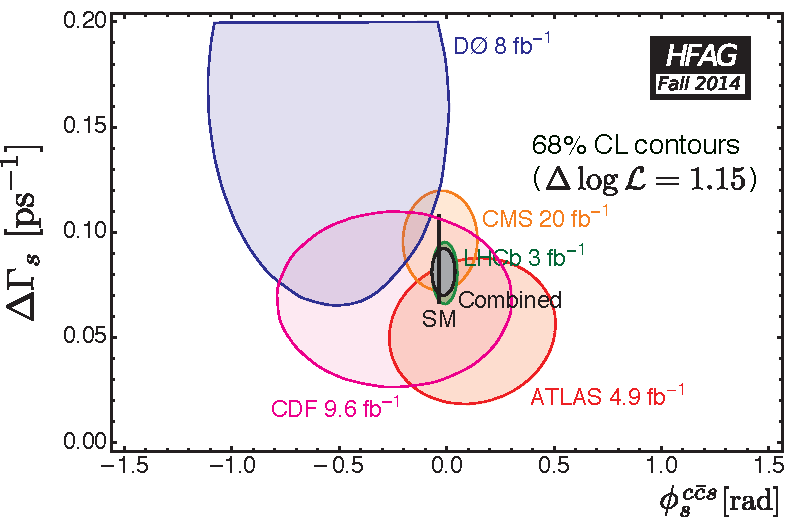
\includegraphics[width=0.49\textwidth]{figures/life_mix/hfag_Fall2014_DGsphis}
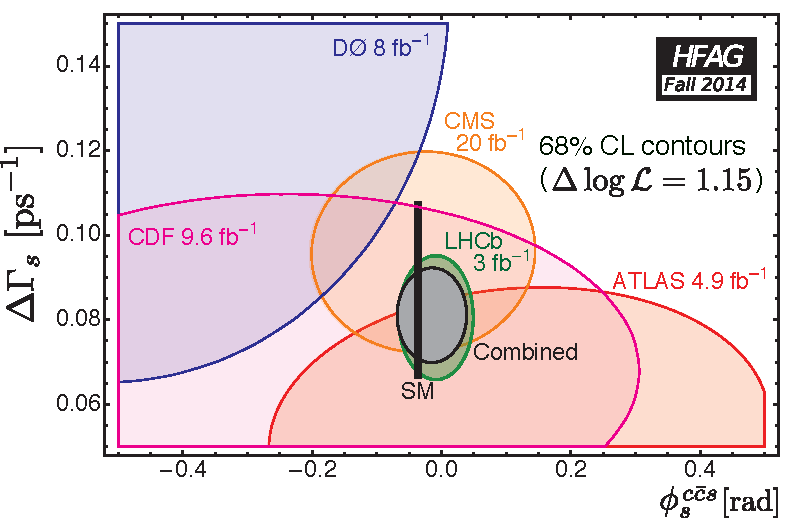
\includegraphics[width=0.49\textwidth]{figures/life_mix/hfag_Fall2014_DGsphis_zoom}
\caption{
Left: 68\% CL regions in \Bs width difference \DGs and weak phase \phiccbars
obtained from individual and combined CDF~\cite{Aaltonen:2012ie,*CDF:2011af,*Aaltonen:2007he_mod,*Aaltonen:2007gf_mod},
\dzero~\cite{Abazov:2011ry,*Abazov_mod:2008fj,*Abazov:2007tx_mod_cont}, ATLAS~\cite{Aad:2014cqa,*Aad:2012kba_cont}, 
CMS~\cite{CMS-PAS-BPH-13-012}
and LHCb~\cite{Aaij:2014zsa,*Aaij:2013oba_supersede2,Aaij:2014dka,*Aaij:2013oba_supersede}
likelihoods of 
$\Bs\to \jpsi\phi$, $\Bs\to \jpsi K^+K^-$ and $\Bs\to\jpsi\pi^+\pi^-$. 
The expectation within the Standard Model~\cite{Charles:2011va_mod,Lenz:2011ti,*Lenz:2006hd}
is shown as the black rectangle.
Right: same, but zoomed on the region of interest.
%  combined contour compared with the 68\% CL (green) and 95\% CL (yellow)
%regions allowed by the measurements of \ASLs and \dms.
}
\labf{DGs_phase}
\end{center}
\end{figure}

We perform a combination of the CDF~\cite{Aaltonen:2012ie,*CDF:2011af,*Aaltonen:2007he_mod,*Aaltonen:2007gf_mod},
\dzero~\cite{Abazov:2011ry,*Abazov_mod:2008fj,*Abazov:2007tx_mod_cont},
ATLAS~\cite{Aad:2014cqa,*Aad:2012kba_cont}, CMS~\cite{CMS-PAS-BPH-13-012}
and LHCb~\cite{Aaij:2014zsa,*Aaij:2013oba_supersede2,Aaij:2014dka,*Aaij:2013oba_supersede}
results summarized in \Table{phisDGsGs}.
%OL2014
%LHCb has performed an internal combination of \phis\ measured using $\Bs \to \jpsi KK$ and $\Bs \to \jpsi\pi\pi$ events~\cite{Aaij:2014zsa,*Aaij:2013oba_supersede2} and obtain  $-0.010\pm0.040(\rm tot)$. 
% BEWARE HARD-CODED!
%We average this with the \phis\ value measured using using $\Bs \to D_s^+ D_s^-$ events~\cite{Aaij:2014ywt}. 
This is done by adding the two-dimensional log profile-likelihood scans of
\DGs and \phiccbars from the four $\Bs\to\jpsi\phi$ ($\Bs\to\jpsi K^+K^-$) analyses and 
a one-dimensional log profile-likelihood of \phiccbars
from the $\Bs\to\jpsi\pi^+\pi^-$ and $\Bs \to D_s^+ D_s^-$ analyses; 
the combined likelihood is then maximized with respect to \DGs and \phiccbars.

In the $\Bs\to\jpsi\phi$ and $\Bs\to\jpsi K^+K^-$ analyses, \phiccbars and \DGs 
come from a simultaneous fit that determines also the \Bs lifetime,
the polarisation amplitudes and strong phases.
While the correlation between \phiccbars and all other parameters is small,
the correlations between \DGs and the polarisation amplitudes are sizeable.
However, since the various experiments use different conventions
for the amplitudes and phases, a full combination including all
correlations is not performed. Instead, our average only takes
into account the correlation between \phiccbars and \DGs.

%2012% where in each case
%2012% the $-$log-likelihood is minimized with respect to all other
%2012% parameters, including \Gs.
%2012% Since the $\Bs\to\jpsi\phi$ two-dimensional scan provided by
%2012% ATLAS~\cite{ATLAS-CONF-2013-039,*Aad:2012kba_cont}
%2012% and LHCb~\cite{Aaij:2013oba,*LHCb:2011aa_mod,*LHCb:2012ad_mod,*LHCb:2011ab_mod,*Aaij:2012nta_mod}
%2012% contain only statistical uncertainties, on each (\DGs, \phiccbars) point,
%2012% we decrease the log-likelihood by the quantity
%2012% \begin{equation}
%2012% \Delta\log{\cal L}^{\rm new}  - \Delta\log{\cal L}^{\rm old} =
%2012% \frac{(\phiccbars-\phi_{s-{\rm min}}^{c\bar{c}s})^2 \sigma_{\phi-\rm syst}^2} 
%2012% {2 \sigma_{\phi-\rm stat}^2 (\sigma_{\phi-\rm stat}^2 + \sigma_{\phi-\rm syst}^2)} +  
%2012% \frac{ (\DGs - \DG_{s-{\rm min}})^2 \sigma_{\DG-{\rm syst}}^2} 
%2012% {2 \sigma_{\DG-\rm stat}^2 (\sigma_{\DG-\rm stat}^2 + \sigma_{\DG-\rm syst}^2)}\,, 
%2012% \end{equation}
%2012% where $\phi_{s-{\rm min}}$ and $\DG_{s-{\rm min}}$ are the values of \phiccbars
%2012% and \DGs at the minimum of the likelihood, and $\sigma_{\phi-\rm stat}$
%2012% ($\sigma_{\DG-\rm stat}$) and $\sigma_{\phi-\rm syst}$ ($\sigma_{\DG-\rm syst}$)
%2012% the statistical and systematic uncertainties on \phiccbars (\DGs).  
%2012% This assumes that the systematic uncertainties are Gaussian
%2012% and independent of \DGs and \phiccbars. % (\DGs, \phiccbars). 
%2012% % Without any additional constraints, we find
%2012% Both the \dzero and CDF log profile-likelihood scans are corrected
%2012% for coverage and include systematic uncertainties.

%OL2014 
In the recent LHCb $\Bs \to \jpsi K^+K^-$ analysis~\cite{Aaij:2014zsa,*Aaij:2013oba_supersede2}, the \phiccbars values are measured for the first time for each polarization of the final state. Since those values are compatible within each other, we still use the unique value of \phiccbars for our world average, corresponding to the one measured by the other-than-LHCb analyses. 
In the same analysis, the statistical correlation coefficient between \phiccbars and $|\lambda|$
(which signals \CP violation in the decay if different from unity) 
is measured to be very small ($-0.02$). We neglect this correlation in our average. 
Furthermore, the statistical correlation coefficient between \phiccbars and \DGs\ is measured to be small $(-0.08)$. When averaging LHCb results of 
$\Bs \to \jpsi K^+K^-$,  $\Bs \to \jpsi \pi^+\pi^-$ and $\Bs \to D_s^+ D_s^-$, we neglect this correlation coefficient (putting it to zero). 
Given the increasing experimental precision, we have also stopped using the two-dimensional $\DGs-\phiccbars$ histograms provided by the CDF and \dzero collaborations: we are now approximating those with two-dimensional Gaussian likelihoods. 

We obtain the individual and combined contours shown in \Fig{DGs_phase}. % (left).
Maximizing the likelihood, we find, as summarized in \Table{phisDGsGs}:  
\begin{eqnarray}
\DGs &=& \hfagDGSCOMB \,, \\    
\phiccbars &=& \hfagPHISCOMB \,.
\labe{phis}
\end{eqnarray}
The above \DGs average is consistent, but highly correlated with the average
of \Eq{DGs_DGsGs}. Our
final recommended average for \DGs is the one of \Eq{DGs_DGsGs}, which 
includes all available information on \DGs. 

In the Standard Model and ignoring sub-leading penguin contributions, 
\phiccbars is expected to be equal to $-2\beta_s$, 
%%% \begin{equation}
%%% (\phiccbars)^{\rm SM} = -2\beta_s \,,
%%% \end{equation}
where
%%% \begin{equation}
$\beta_s = \arg\left[-\left(V_{ts}V^*_{tb}\right)/\left(V_{cs}V^*_{cb}\right)\right]$ % \,.
%%% %= 0.036 \pm 0.002 \approx 0.04.
%%% \end{equation}
is a phase analogous to the angle $\beta$ of the usual CKM
unitarity triangle (aside from a sign change). % the negative sign.
% (resulting in a positive angle in the Standard Model).
An indirect determination via global fits to experimental data
gives~\cite{Charles:2011va_mod}
\begin{equation}
%(\phiccbars)^{\rm SM} = -2\beta_s = -0.0363^{+0.0012}_{-0.0014} \,.
(\phiccbars)^{\rm SM} = -2\beta_s = \hfagPHISSM \,.
\labe{phisSM}
\end{equation}
The average value of \phiccbars from \Eq{phis} is consistent with this
Standard Model expectation.

New physics could contribute to \phiccbars. Assuming that new physics only 
enters in $M_{12}$ (rather than in $\Gamma_{12}$),
one can write~\cite{Lenz:2011ti,*Lenz:2006hd}
%%% The same additional contribution due to new physics would show up in this
%%% observed phase~\cite{Lenz:2011ti,*Lenz:2006hd}, {\it i.e.}
\begin{equation}
\phiccbars = -  2\beta_s + \phi_{12}^{\rm NP} \,,
\end{equation}
where the new physics phase $\phi_{12}^{\rm NP}$ is the same as that appearing in \Eq{phi12NP}.
In this case
\begin{equation}
\phi_{12} = % \phi_{12}^{\rm SM}+ \phi_{12}^{\rm NP} =
\phi_{12}^{\rm SM} +2\beta_s + \phiccbars = \hfagPHISTWELVE \,,
\end{equation}
where the numerical estimation was performed with the values of \Eqsss{phis12SM}{phisSM}{phis}.
% and \Eq{ASLS_tanphi12} then provides a relation between \DGs and \phiccbars, 
% based on the measured values of \ASLs and \dms (\Eqss{ASLS}{dms}) 
% as well as the expectations
% for $\phi_{12}^{\rm SM}$ and $-2\beta_s$.
% The allowed region in the (\DGs, \phiccbars) plane is shown in 
% \Fig{DGs_phase_old} (right), where it is compared both with the
% direct measurement of \DGs and \phiccbars,
% and with the Standard Model expectations. 
% No inconsistency is observed between all these data.
This can serve as a reference value to which the measurement of \Eq{tanphi12} can be compared. 


%%% In \Fig{DGs_phase} (right), this result is compared to the 
%%% constraint provided by the world-average \Bs semileptonic asymmetry of
%%% \Eq{ASLS} and the world-average mass difference \dms of \Eq{dms} through~\cite{Beneke:2003az}:
%%% \begin{equation}
%%% \ASLs = 
%%% \Im \left(\frac{\Gamma^{12}_s}{M^{12}_s} \right) + {\cal O} \left( \frac{\Gamma_{12}}{M_{12}} \right)^2 =
%%% \frac{\DGs}{\dms}\tan\phi_{12} + {\cal O} \left( \frac{\Gamma_{12}}{M_{12}} \right)^2 \,,
%%% \end{equation}
%%% where, ignoring penguin contributions and using the Standard Model values of $\phi_{12}^{\rm SM}$ and $-2\beta_s$, we have
%%% \begin{equation}
%%% \phi_{12} = % \phi_{12}^{\rm SM}+ \phi_{12}^{\rm NP} =
%%% \phi_{12}^{\rm SM} +2\beta_s + \phiccbars \,.
%%% \end{equation}

% allowing the extraction of \phiccbars\ from \ASLs\ given the SM
% values of $\phi_{12}^{\mathrm SM}$ and $2\beta_s$. 
%
% And the result are
% citation to be update to should be  Lenz, arXiv:1102.4274
% \begin{eqnarray}
% \DGs &=& \hfagDGSCOMBCON \,, \\    
% \phiccbars =  &=& \hfagPHISCOMBCON \,.
% \end{eqnarray}

% UNDER DISCUSSION:
% In addition, we introduce the constraints due to the effective lifetime measured in $\hbox{\Bs} \to K^+K^-$~\cite{Aaij:2011kn},
% and $\hbox{\Bs} \to \jpsi f_0(980)$~\cite{Aaltonen:2011nk}, using \Eqss{tauf_fleisch,ADG}.
% We find: 
% \begin{eqnarray}
% \DGs &=&   ~~TO~BE~UPDATED \\
% \phiccbars =  &=&  ~~TO~BE~UPDATED 
% \end{eqnarray}.


% OL comments the following temporary: 
\comment{

For non-zero $|\Gamma_{12}|$, analysis of the time-dependent
decay \particle{\Bs \to \jpsi\phi} can measure
the weak phase.  Including information on the \Bs flavour at production
time via flavour tagging improves precision and also resolves the 
sign ambiguity on the weak phase angle for a given \DGs.
Both CDF~\cite{CDF:2011af,*Aaltonen:2007he_mod,*Aaltonen:2007gf_mod} 
and \dzero~\cite{Abazov:2011ry,*Abazov_mod:2008fj,*Abazov:2007tx_mod_cont} have performed 
such analyses and measure the same observed phase that we denote
$\phi_s^{\jpsi \phi} = -2\beta_s^{\jpsi \phi}$ to reflect
the different conventions of the experiments.

Under the assumption of non-zero $\phi_s^{\jpsi\phi}$, 
in addition to the result listed
in \Table{dgammat}, 
the \dzero collaboration~\cite{Abazov:2011ry,*Abazov_mod:2008fj,*Abazov:2007tx_mod_cont}  has also made simultaneous
fits allowing $\phi_s^{\jpsi\phi}$ to float while weakly 
constraining the strong phases, $\delta_i$ to find: 
\begin{eqnarray}
\DGs &=& +0.19 \pm 0.07 ^{+0.02}_{-0.01}~{\mathrm{ps}}^{-1}\,,  \\ 
\bar{\tau}(\Bs) &= &1/\Gs = 1.52 \pm 0.06~{\mathrm{ps}}\,,  \\
\phi_s^{\jpsi\phi} &=& -0.57 ^{+0.24+0.07}_{-0.30-0.02} \,. 
\end{eqnarray}
If the SM value of $\phi_s^{\jpsi\phi} = -0.04$ is assumed, a probability of 
6.6\% to obtain a value of $\phi_s^{\jpsi\phi}$ lower than $-0.57$ is
found.

The CDF 
analysis~\cite{CDF:2011af,*Aaltonen:2007he_mod,*Aaltonen:2007gf_mod} 
reports confidence regions
in the two-dimensional space of $2\beta_s^{\jpsi\phi}$ and \DGs.
They present a Feldman-Cousins confidence interval of $2\beta_s^{\jpsi\phi}$
where \DGs is treated as a nuisance parameter:
\begin{equation}
2\beta_s^{\jpsi\phi} = -\phi_s^{\jpsi\phi} \in [0.56,2.58]~{\mathrm{at~68\%~CL}}.
\end{equation}
Only a confidence range is quoted and a  point 
estimate is not given since biases were observed in the analysis.
Assuming the SM predictions for $2\beta_s$ and \DGs, they find
that the probability of a deviation as large as the level of the 
observed data is 7\%.
Note that CDF has very recently made a preliminary update~\cite{CDFnote10778:2012,*CDFnote10778:2012_cont}
to their
\particle{\Bs \to \jpsi\phi} analysis to an
integrated luminosity of 5.2~fb$^{-1}$ indicating a best-fit
confidence interval of:
\begin{equation}
2\beta_s^{\jpsi\phi} = -\phi_s^{\jpsi\phi} 
\in [0.04,1.04] \cup [2.16,3.10]~{\mathrm{at~68\%~CL}},
\end{equation}
where the probability
of a larger deviation from the SM prediction is 44\% or $0.8\,\sigma$.
However, this new result has not yet been used in the combinations
below.

Given the consistency of these two measurements of the weak phase,
as well as their
deviations from the SM, there is interest in combining the results and
using in global fits, \eg\ see \Ref{Bona:2008jn}.
To allow a combination on equal footing, the \dzero collaboration
has redone their fits~\cite{D0web:2009} 
allowing  strong phase values, $\delta_i$, to float
as in the CDF analysis.
Ensemble studies to test confidence level coverage were performed 
by both collaborations and used to adjust likelihood
values to correspond to the usual Gaussian confidence levels. 
Two-dimensional likelihoods were 
combined~\cite{CDFnote9787:2009,D0Note5928:2009}
with the result shown in 
\Fig{DGs_phase}(a).  
After the combination, consistency  
of the best fit values for $\phi_s^{\jpsi\phi} = -2\beta_s^{\jpsi\phi}$ with
SM predictions is at the level of $\hfagNSIGMASM\,\sigma$, with numerical results
for the two solutions given below.
Despite possible biases in the CDF input, point estimates are still
presented and the confidence level regions are straight projections
onto the \DGs or phase angle axes.
\begin{eqnarray}
\DGs &=& \hfagDGSCOMB \,, \\
\phi_s^{\jpsi\phi} = -2\beta_s^{\jpsi\phi} &=& \hfagPHISCOMB \,.
\end{eqnarray}

A comparison between
the above sum of the
CDF and \dzero likelihoods 
and the world average \Bs semileptonic asymmetry of
%5 i.e., to the flavour-specific
% \Bs lifetime world average of \Eq{tau_fs} 
%through \Eq{fslife_const} and to
%the world average \Bs semileptonic asymmetry of 
\Eq{ASLS} through~\cite{Beneke:2003az}:
\begin{equation}
\ASLs = 
\frac{|\Gamma^{12}_s|}{|M^{12}_s|}\sin\phi_s = \frac{\DGs}{\dms}\tan\phi_s
\end{equation}
is also made and shown in 
\Fig{DGs_phase}(a).
Consistency between the two is observed, and the value
of \ASLs is applied as a constraint
resulting in the
confidence level regions 
shown in \Fig{DGs_phase}(b)
including the region delineated by new physics traced by 
the relation of \Eq{new_phys_phase}. Numerical results for the 
two solutions are:
\begin{eqnarray}
\DGs &=& \hfagDGSCOMBCON \,, \\
\phi_s^{\jpsi\phi} = -2\beta_s^{\jpsi\phi} &=& \hfagPHISCOMBCON \,.
\end{eqnarray}
with a consistency
of the best fit values with
SM predictions of $2\beta_s$ at the level of $\hfagNSIGMASMCON\,\sigma$.


}

%end_2009% Finally, additional constraints are added due to
%end_2009% the flavour-specific
%end_2009% \Bs lifetime world average of \Eq{tau_fs} 
%end_2009% through \Eq{fslife_const}, the \CP-event lifetime
%end_2009% of \Eq{tau_CPeven},
%end_2009% and the world average of the branching fraction
%end_2009% $\BR{B^0_s \to D_s^{(*)+} D_s^{(*)-}}$
%end_2009% through~\cite{Dunietz:2000cr}:
%end_2009% \begin{eqnarray}
%end_2009% 2{\cal{B}}(B^0_s \to D_s^{(*)+}D_s^{(*)-}) \simeq
%end_2009% \DGs^{\mathrm{CP}}
%end_2009% \left[
%end_2009% \frac{\frac{1}{1 - 2x_f} + \cos\phi_s}{2 \Gamma_{\rm L}} +
%end_2009% \frac{\frac{1}{1 - 2x_f} - \cos\phi_s}{2 \Gamma_{\rm H}}
%end_2009% \right]\,.
%end_2009% \end{eqnarray}
%end_2009% Here $x_f$ is the fraction of the \CP-odd component
%end_2009% of the decay.
%end_2009% To apply this as a constraint, we expand the above expression 
%end_2009% to second order,
%end_2009% \begin{eqnarray}
%end_2009% 2{\cal{B}}(B^0_s \to D_s^{(*)+}D_s^{(*)-}) \simeq
%end_2009% \frac{\DGs }{\Gs \cos \phi_s}
%end_2009% \left[
%end_2009% \frac{1}{1 - 2x_f} - \frac{\DGs \cos \phi_s}{2 \Gs}
%end_2009% \right]\,,
%end_2009% \end{eqnarray}
%end_2009% and use the world average of the branching ratio of \Table{dGsBr}.
%end_2009% Numerical results following these final constraints are:

% RvK: tentatively remove this figure and results for now, and given the
% increased inconsistency of tau(Bd) and tau(Bs).
% \begin{figure}
% \begin{center}
% \includegraphics[width=0.45\textwidth]{figures/life_mix/win05_semi_taubd}
% \caption{\DGs combination results with one-sigma contours
% ($\Delta\log\mathcal{L} = 0.5$) shown for \DGGs versus
% $\bar{\tau}(\Bs) = 1/\Gs$.
% The contour labelled ``Direct" is the result of the combination of
% most measurements of \Table{dgammat}, the blue band is the one-sigma
% contour due to the world average of flavour-specific measurements,
% the red vertical band the one-sigma constraint of
% $\bar{\tau}(\Bs) = 1/\Gs = \tau(\Bd) = 1/\Gd$ (with an additional
% error added in quadrature),
% and the shaded region the combination.}
% \labf{DGscon}
% \end{center}
% \end{figure}
%
% The {\em average} \Bs and \Bd
% lifetimes are predicted to be equal within
% 1\%~\cite{Beneke:1996gn,*Keum:1998fd,Gabbiani:2004tp}
% and in the past, an additional constraint was applied 
% by setting
% $\Gs = \Gd$, \ie, $1/\Gs = \tau(\Bd)$,
% where $\tau(\Bd) = \hfagTAUBD$ is the world average of experimental results,
% including a relative 1\% theoretical uncertainty added
% in quadrature with the indicated experimental error.
% However, with the increased inconsistency of
% the measured values of $1/\Gs= \bar{\tau}(\Bs)$ and $\tau(\Bd)$
% at the level of $\hfagRTAUBSMEANCsig\,\sigma$,
% this constraint is no longer applied. 
% this constraint is now less valid and is not presented here.


